\documentclass{beamer}
%
% Choose how your presentation looks.
%
% For more themes, color themes and font themes, see:
% http://deic.uab.es/~iblanes/beamer_gallery/index_by_theme.html
%
\mode<presentation>
{
  \usetheme{Boadilla}      % or try Darmstadt, Madrid, Warsaw, ...
  \usecolortheme{beaver} % or try albatross, beaver, crane, ...
  \usefonttheme{default}  % or try serif, structurebold, ...
  \setbeamertemplate{navigation symbols}{}
  \setbeamertemplate{caption}[numbered]
  
} 

\usepackage{xcolor,colortbl}
\usepackage[english]{babel}
\usepackage[utf8x]{inputenc}
\usepackage{courier}
\usepackage{dsfont}
\usepackage{verbatim} 
\usepackage{enumerate}
\usepackage{tikz}
\usepackage{multirow}
\usepackage{venndiagram}
\usepackage{epigraph} 
%\usepackage{xcolor}
\usepackage{makecell}

%\usepackage{enumitem}

\usepackage{hyperref}
\hypersetup{
    colorlinks=true,
    linkcolor=blue,
    filecolor=magenta,      
    urlcolor=cyan,
}

% R stuff!
\usepackage{listings}
\definecolor{codegreen}{rgb}{0,0.6,0}
\definecolor{codegray}{rgb}{0.5,0.5,0.5}
\definecolor{codepurple}{rgb}{0.58,0,0.82}
\definecolor{backcolour}{rgb}{0.95,0.95,0.92}

\lstdefinestyle{mystyle}{
    backgroundcolor=\color{backcolour},    
    commentstyle=\color{codegreen},
    keywordstyle=\color{black},
    numberstyle=\tiny\color{codegray},
    stringstyle=\color{codepurple},
    basicstyle=\ttfamily\footnotesize,
    breakatwhitespace=false,         
    breaklines=true,                 
    captionpos=b,                    
    keepspaces=true,                 
    numbers=left,                    
    numbersep=5pt,                  
    showspaces=false,                
    showstringspaces=false,
    showtabs=false,                  
    tabsize=2
}

\lstset{style=mystyle}


\setbeamertemplate{enumerate items}[default]
\setbeamertemplate{itemize item}[triangle]

%\setitemize{label=\usebeamerfont*{itemize item}%
%  \usebeamercolor[fg]{itemize item}
%  \usebeamertemplate{itemize item}}



\title[Introduction to Statistics]{Confidence Intervals for Proportions}
\subtitle{}
\author{Grinnell College}
\date{}

\graphicspath{{img/}}

\begin{document}

\begin{frame}
  \titlepage
\end{frame}

\begin{frame}{Review}
We have seen how to make CI's for pop. means or the diff. in pop. means \vspace{6mm}

Confidence intervals will always have the following form:
\begin{align*}
    \text{statistic} \pm C \times \text{SE}
\end{align*} \vspace{6mm}

There is a quick-guide available on the course page that will be a good reference for you as we continue.
\end{frame}

\begin{frame}{Outline}
Today we will learn how to work with proportions.
\begin{itemize}
    \item CI for a single population proportion (p)
    \item CI for a difference in population proportions (p$_1$ - p$_2$).
\end{itemize} \vspace{6mm}

These slides will not be extensive. Once you know how to make CI's for means like you have seen, proportions are not much different.
\end{frame}

\begin{frame}{Means vs. Proportions}
Let's think back to what type of variables we are working with. \vspace{6mm}

\textbf{Quantitative Variables}
\begin{itemize}
    \item use means (and standard deviation) to describe the population
    \item one group $\rightarrow$ one mean ($\mu$)
    \item two groups $\rightarrow$ diff. in means ($\mu_1 - \mu_2$)
\end{itemize} \vspace{6mm}

\textbf{Categorical Variables}
\begin{itemize}
    \item use the proportion of a category to describe the population
    \item one group $\rightarrow$ one proportion (p)
    \item two groups $\rightarrow$ diff. in proportions (p$_1$ - p$_2$)
\end{itemize}
\end{frame}

\begin{frame}{Proportions -- Examples}
Let's say we want to find out if a coin is "fair." We could flip the coin a whole bunch of times
\begin{itemize}
    \item outcomes are Heads or Tails $\rightarrow$ categorical
    \item record the 'proportion of heads'
    \item should be close to 0.5 if coin is fair
\end{itemize} \vspace{8mm}

In an election year in the U.S., political campaigns (and political groups in general) are interested in finding out how people are going to vote
\begin{itemize}
    \item who someone will vote for $\rightarrow$ categorical
    \item we want to estimate 'proportion who will vote for a candidate'
\end{itemize} \vspace{3mm}
\end{frame}

\begin{frame}{CIs for Proportions}
We will now go through and explain the logic related to how CI's for proportions was developed.
\end{frame}

\begin{frame}{Relationship between Means and Proportions}
There is an interesting relationship between means and proportions \vspace{4mm}

For example, consider taking a fair coin and flipping it 10 times. How many heads would you expect to see?
\end{frame}



\begin{frame}{Relationship between Means and Proportions}
\footnotesize
Say we flip the coin 10 times and get the following sample $\mathcal{S}$.

\begin{align*}
\mathcal{S} &= \{H, H, T, T, H, T, H, T, T, T\} \\
X &= \{1, 1, 0, 0, 1, 0, 1, 0, 0, 0 \}
\end{align*}
\begin{columns}

  \begin{column}{0.45\textwidth}
 We can find the \textit{proportion} of heads from our sample $\mathcal{S}$ by simply taking the total number of heads and dividing by the total number of flips, giving
 \begin{align*}
 \hat{p} = \frac{4}{10}
 \end{align*}
However, if we consider $X$, which defines $H$ as $1$ and $T$ as $0$, we can also find the sample mean:
\begin{align*}
\overline{x} &= \frac{1}{10} \sum_{i=1}^n x_i \\
&= 0.4
\end{align*}
  \end{column}
  \begin{column}{0.45\textwidth}
\begin{center}
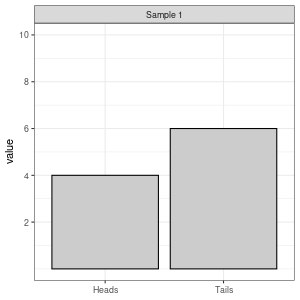
\includegraphics[scale=0.5]{10_flip.png}
\end{center}
  \end{column}

\end{columns}
\end{frame}

\begin{frame}{Repeated Samples}
\begin{center}
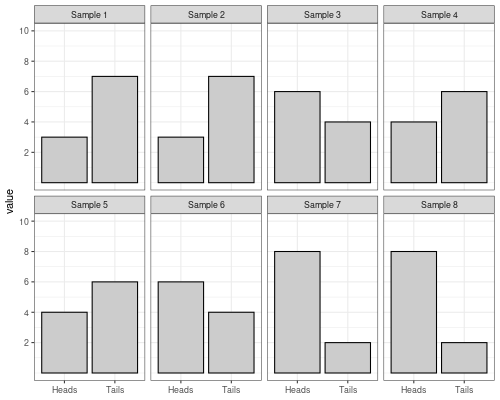
\includegraphics[scale=0.5]{mult_coin_flip.png}
\end{center}
\end{frame}

\begin{frame}{Sampling Distr. for the Proportion of Heads}
\begin{center}
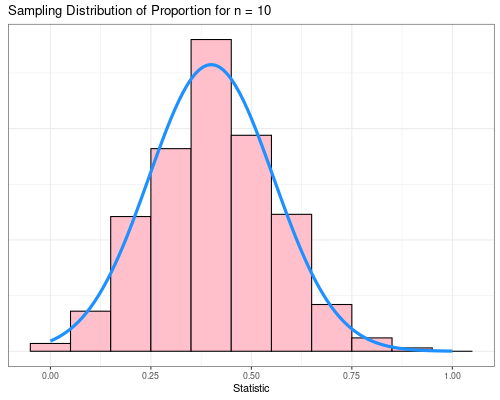
\includegraphics[scale=0.5]{p_samp_dist.png}
\end{center}
\begin{itemize}
    \item What does this look like?
\end{itemize}
\end{frame}

\begin{frame}{Central Limit Theorem}
For a sample with one proportion, the sampling distribution of our proportion statistic, $\hat{p}$ is approximately

\begin{align*}
\hat{p} \sim  N \left( p, \ \sqrt{\frac{p(1-p)}{n}} \right)
\end{align*}

There a few rules of thumb relating to the size and the proportion:
\begin{enumerate}
\item $n \times p \geq 10$
\item $n \times (1-p) \geq 10$
\end{enumerate}
\vspace{3mm}
In particular, it is often difficult to estimate proportions precisely that are near the boundaries (0 and 1)
\end{frame}

\begin{frame}{Back to CI's}
So... the sampling dist. for a population mean looks Normal!
\begin{itemize}
    \item we used this result to make CIs for means
    \item we are going to use it for CIs for proportions too
\end{itemize} \vspace{6mm}


Confidence intervals will always have the following form:
\begin{align*}
    \text{statistic} \pm C \times \text{SE}
\end{align*}


\begin{itemize}
    \item C will be determined by the confidence just like we've seen
    \item 95\% confidence $\rightarrow$ C=1.96
    \item we will \textbf{always} use the normal distribution for proportions
\end{itemize}
\end{frame}

\begin{frame}{CI for a population proportion}
\begin{align*}
    \text{statistic} \pm C \times \text{SE}
\end{align*}

Want to estimate the population proportion p. Use what we have
\begin{itemize}
    \item statistic = $\widehat{p}$
\end{itemize} \vspace{8mm}

We can get the SE from the CLT result for proportions
\begin{align*}
\hat{p} \sim  N \left( p, \ \sqrt{\frac{p(1-p)}{n}} \right)
\end{align*}
\begin{itemize}

    \item we don't know the value for p $\rightarrow$ SE = $\sqrt{\frac{\widehat{p}(1-\widehat{p})}{n}}$
\end{itemize}
\end{frame}

\begin{frame}{CI for a population proportion}
Our final formula for estimating p (a population proportion):
\begin{align*}
    \widehat{p} \pm z^* \times \sqrt{\frac{\widehat{p}(1-\widehat{p})}{n}}
\end{align*}

\begin{itemize}
    \item $\widehat{p}$ is the sample proportion
    \item n is our sample size
    \item $z^*$ is the appropriate value from the normal distribution that gives us the Confidence \% that we want
    \begin{itemize}
        \item 95\% Confidence $\rightarrow z^* = 1.96$
        \item 80\% Confidence $\rightarrow z^* = 1.282$
        \item 90\% Confidence $\rightarrow z^* = 1.645$
        \item 99\% Confidence $\rightarrow z^* = 2.576$
    \end{itemize}
\end{itemize}
\end{frame}

\begin{frame}{CI for proportion -- Conditions}
The conditions required for the CI to work well for a pop. proportion:

\begin{itemize}
    \item Random sample
    \item $n \times p \geq 10$ (Success Condition)
    \item $n \times (1-p) \geq 10$ (Failure Condition)
\end{itemize} \vspace{6mm}

Success and Failure conditions get their name from counting the \# of successes and failures respectively. When checking conditions:

\begin{itemize}
    \item say that each condition is "met" or "not met"
    \item i.e.: random sample (met / not met)
    \item i.e.: Success condition (met / not met)
    \item i.e.: Failure condition (met / not met)
\end{itemize}
\end{frame}

\begin{frame}{Example}
\small
In a study conducted by Johns Hopkins University researchers
investigated the survival of babies born prematurely. They searched
their hospital’s medical records and found 39 babies born at 25
weeks gestation (15 weeks early), 31 of these babies went on to
survive at least 6 months. With your group:
\begin{enumerate}
\item Use a normal approximation to construct a 95\% confidence interval estimate for the true proportions of babies born at 25 weeks gestation that are expected to survive
\item An article on Wikipedia suggests that 70\% of babies born at a gestation period of 25 weeks survive. Is this claim consistent with the Johns Hopkins study?
\end{enumerate}
\end{frame}

\begin{frame}{Example}
\small
\begin{enumerate}
\item We find that
\begin{align*}
\hat{p} &= \frac{31}{39} = 0.795 \\
SE &= \sqrt{\frac{0.795(1-0.795)}{39}} = 0.065
\end{align*}
From here, we found our 95\% CI:
\begin{align*}
0.795 \pm 1.96 \times 0.065 = (0.668, 0.922)
\end{align*}
\item As 0.7 is contained within our constructed 95\% CI, it is consistent with the results of the study by Johns Hopkins
\end{enumerate}
\end{frame}

\begin{frame}{Difference in Proportions}
Just like how we sometimes wanted to find a difference in means... we can do the same thing for proportions
\begin{itemize}
    \item need to be careful that we are not confusing ourselves
\end{itemize} \vspace{4mm}

When do we want to estimate a proportion vs. difference in proportions?
\begin{itemize}
    \item we need to have 2 groups defined by a 2nd variable
    \item this is not the same as having multiple categories for the categorical variable we are working with
\end{itemize} \vspace{4mm}
\end{frame}

\begin{frame}{Difference in Proportions}
Example: Coin flips
\begin{itemize}
    \item We can estimate proportion of heads or proportion of tails
    \item if we know one, we know the other by default
    \item Heads/Tails are different categories of the variable of interest
    \item we do not need to estimate a difference in proportions
\end{itemize} \vspace{8mm}

Example: New medical treatment for headaches
\begin{itemize}
    \item We can compare survival rates between treatment \& control groups
    \item 2nd variable: whether someone received the treatment (Yes/No)
    \item two groups $\rightarrow$ need to estimate a \textit{difference} in means
\end{itemize}
\end{frame}

\begin{frame}{CI for difference in population proportions}
\begin{align*}
    \text{statistic} \pm C \times \text{SE}
\end{align*}

Want to estimate the difference in population proportions ($p_1 - p_2$)
\begin{itemize}
    \item statistic = $\widehat{p}_1 - \widehat{p}_2$
\end{itemize} \vspace{8mm}

\begin{itemize}
    \item SE = $\sqrt{\frac{\widehat{p}_1(1-\widehat{p}_1)}{n_1} + \frac{\widehat{p}_2(1-\widehat{p}_2)}{n_2}}$
\end{itemize}
\end{frame}


\begin{frame}{CI for difference in population proportions}
Our final formula for estimating $p_1 - p_2$ (diff. in pop. proportions):
\begin{align*}
    (\widehat{p}_1 - \widehat{p}_2) \pm z^* \times \sqrt{\frac{\widehat{p}_1(1-\widehat{p}_1)}{n_1} + \frac{\widehat{p}_2(1-\widehat{p}_2)}{n_2}}
\end{align*}

\begin{itemize}
    \item $\widehat{p}_1$, $\widehat{p}_2$ are the sample proportions
    \item $n_1$, $n_2$ are the sample sizes
    \item $z^*$ is the appropriate value from the normal distribution that gives us the Confidence \% that we want
    \begin{itemize}
        \item 95\% Confidence $\rightarrow z^* = 1.96$
        \item 80\% Confidence $\rightarrow z^* = 1.282$
        \item 90\% Confidence $\rightarrow z^* = 1.645$
        \item 99\% Confidence $\rightarrow z^* = 2.576$
    \end{itemize}
\end{itemize}
\end{frame}

\begin{frame}{CI for diff. in proportions -- Conditions}
The conditions required for the CI to work well for a difference in proportions are:

\begin{itemize}
    \item Groups are independent of each other (not influencing each other)
    \begin{itemize}
        \item satisfied if we have a random sample
    \end{itemize}
    \item $n_1 \times p_1 \geq 10$
    \item $n_1 \times (1-p_1) \geq 10$
    \item $n_2 \times p_2 \geq 10$
    \item $n_2 \times (1-p_2) \geq 10$
\end{itemize}
    
\end{frame}

%%%%%%%%%%%%%%%%

%\begin{frame}
%\begin{columns}
%
%  \begin{column}{0.45\textwidth}
%%
%  \end{column}
%  \begin{column}{0.45\textwidth}
%%
%  \end{column}
%
%\end{columns}
%\end{frame}


\end{document}


